
%(BEGIN_QUESTION)
% Copyright 2010, Tony R. Kuphaldt, released under the Creative Commons Attribution License (v 1.0)
% This means you may do almost anything with this work of mine, so long as you give me proper credit

The following relay circuit has a problem.  The LED lamp never comes on, regardless of the amount of pressure or temperature sensed by the switches:

$$\includegraphics[width=15.5cm]{i02231x01.eps}$$

Using a digital multimeter, you measure 23.5 volts DC between points {\bf D} and {\bf B} when the temperature is 102 degrees F and the pressure is 18 PSI.

\vskip 10pt

Identify the likelihood of each specified fault for this circuit.  Consider each fault one at a time (i.e. no coincidental faults), determining whether or not each fault could independently account for {\it all} measurements and symptoms in this circuit.

% No blank lines allowed between lines of an \halign structure!
% I use comments (%) instead, so that TeX doesn't choke.

$$\vbox{\offinterlineskip
\halign{\strut
\vrule \quad\hfil # \ \hfil & 
\vrule \quad\hfil # \ \hfil & 
\vrule \quad\hfil # \ \hfil \vrule \cr
\noalign{\hrule}
%
% First row
{\bf Fault} & {\bf Possible} & {\bf Impossible} \cr
%
\noalign{\hrule}
%
% Another row
Pressure switch failed open &  &  \cr
%
\noalign{\hrule}
%
% Another row
Temperature switch failed open &  &  \cr
%
\noalign{\hrule}
%
% Another row
0.5 amp fuse blown &  &  \cr
%
\noalign{\hrule}
%
% Another row
1 amp fuse blown &  &  \cr
%
\noalign{\hrule}
%
% Another row
Relay coil failed open &  &  \cr
%
\noalign{\hrule}
%
% Another row
Pressure switch failed shorted &  &  \cr
%
\noalign{\hrule}
%
% Another row
Temperature switch failed shorted &  &  \cr
%
\noalign{\hrule}
%
% Another row
Relay coil failed shorted &  &  \cr
%
\noalign{\hrule}
} % End of \halign 
}$$ % End of \vbox

Finally, explain why no further diagnostic tests or measurements are necessary to identify the location and nature of the fault.

\vfil 

\underbar{file i02231}
\eject
%(END_QUESTION)





%(BEGIN_ANSWER)

This is a graded question -- no answers or hints given!

%(END_ANSWER)





%(BEGIN_NOTES)

We should not be seeing voltage between test points D and B with the pressure above 15 PSI, because this amount of pressure should force the pressure switch open and therefore cut power to the relay coil.  The fact we have voltage there tells us the pressure switch is not opening, which explains why the LED will not energize (the energized relay holds its NC contact open, cutting power to the LED).  At this point, we have our solution: the one fault (shorted pressure switch) explains all the observed data, as no other fault can.

% No blank lines allowed between lines of an \halign structure!
% I use comments (%) instead, so that TeX doesn't choke.

$$\vbox{\offinterlineskip
\halign{\strut
\vrule \quad\hfil # \ \hfil & 
\vrule \quad\hfil # \ \hfil & 
\vrule \quad\hfil # \ \hfil \vrule \cr
\noalign{\hrule}
%
% First row
{\bf Fault} & {\bf Possible} & {\bf Impossible} \cr
%
\noalign{\hrule}
%
% Another row
Pressure switch failed open &  & $\surd$ \cr
%
\noalign{\hrule}
%
% Another row
Temperature switch failed open &  & $\surd$ \cr
%
\noalign{\hrule}
%
% Another row
0.5 amp fuse blown &  & $\surd$ \cr
%
\noalign{\hrule}
%
% Another row
1 amp fuse blown &  & $\surd$ \cr
%
\noalign{\hrule}
%
% Another row
Relay coil failed open &  & $\surd$ \cr
%
\noalign{\hrule}
%
% Another row
Pressure switch failed shorted & $\surd$ &  \cr
%
\noalign{\hrule}
%
% Another row
Temperature switch failed shorted &  & $\surd$ \cr
%
\noalign{\hrule}
%
% Another row
Relay coil failed shorted &  & $\surd$ \cr
%
\noalign{\hrule}
} % End of \halign 
}$$ % End of \vbox

Sometimes students will get confused over the ``normal'' statuses of the switch contacts within this circuit.  Remember that switch contacts are {\it always} drawn in their ``normal'' states {\it as defined by the manufacturer}, which is to say when each switch is in its minimum-stimulus condition.  Thus, the NC pressure switch is drawn as closed when at rest (i.e. no applied pressure), the NC relay contact connected to the LED is drawn as closed when at rest (i.e. coil unpowered), and the NO temperature switch is drawn as open when at rest (i.e. cold).  These symbols must be interpreted {\it independently} of one another, just as the manufacturer labels them.  

Bear in mind that these switch contact states may not be the actual states of the switches when they are all put together and working in this system.  For example, when the pressure and temperature switches in this system are both in their minimum-stimulus conditions (at rest), the relay will in fact be {\it energized}, causing the NC relay contact to be forced open (in its {\it actuated}, or {\it non-resting} state)!

The fact that the LED never lights up suggests to us that the relay switch contact may be held open (i.e. actuated).  This could be caused by the coil receiving power at all times.  Our measurement of 23.5 volts between points D and B seems to confirm this hypothesis, which is why we must suspect the pressure switch to be at fault: sending power to the relay coil even when it should not.


%INDEX% Troubleshooting review: electric circuits

%(END_NOTES)


